\graphicspath{{figs/3c}}

\chapter{Uncertainty Applications}
\section{Monte-Carlo Dropout on MNIST}
In this section, we focus on training a model using Monte Carlo Dropout (MC Dropout) on the MNIST dataset. Our primary aim was to identify the most uncertain samples. To do this, we used the variation ratio metric, which effectively measures epistemic uncertainty and is straightforward to calculate. For a given image, denoted as $ \mathbf{x} $, we perform $ T $ stochastic forward passes through the model and record the predicted labels. We then determine the frequency $ f^{c^\star }_\mathbf{x} $ of the most common label ($ c^\star $) across the $ T $ passes. The variation ratio for image $ \mathbf{x} $ is calculated using the formula:
\[
    \text{var-ratio}[\mathbf{x}] = 1 - \frac{f^{c^\star }_\mathbf{x}}{T}
.\]
This formula provides a quantitative measure of uncertainty for an image.


\paragraph*{1.1. What can you say about the images themselfs? How do the histograms along them helps to explain failure cases? Finally, how do probabilities distribution of random images compare to the previous top uncertain images?}

In this experiment, we used a LeNet-5 styled model with Monte-Carlo dropout variational inference. The model was train on MNIST for 20 epoch using cross-entropy in a clasical way. Then we use the model to compute the variation ratios for each test image. This permit to retrieve images by them uncertainty. That what have been done in \Cref{fig:varratio_certain,fig:varratio_certain}, they denote five measurement over the models probabilities outputs for two certain and uncertain images. To sum up the behaviour of the logit over the $ T=100 $ stochastic forward pass, we used histograms that display three distribution : the distribution of the mean of the outputs probabilities, the distribution of the max probability and the distribution of the probability of a particular class (the most predicted class for the first column, the ground truth class in the second column, a another different class the the third column).

Those histogram represent how the output probabilities vary other $ T=100 $ draw. If the model is not confident in its prediction, this will be reflected by high variation in probabilities between each draw and so, histograms will be more sparce.

\Cref{fig:varratio_certain} present images caracterized as certain by the model. With our humain eye, they seem to clearly represent their denoted class. About the presented distributions, they are composed of a single peaked, this mean that we approximatly draw the same value every time, meaning that the model is pretty confident about it's output. 

In the other hand \Cref{fig:varratio_uncertain} present the same thing for images caracterized as uncertain by the model. With our humain eye, numbers seem much more ambiguous. We can see much more spreaded distribution. The distribution of the mean probabilities can sometime be pretty low, meaning that the model is unconfident, or sometime really high, meaning the model is over-confident on a uncertain image. We observe the same behaviour for the distribution of the maximum probability. For the distribution of the probabilities for the ground thruth class and the predicted class, we can see that the distribution is really spreaded (large std), translating a unconfident prediction for those classes. Samples for another class have less variance but it still more than in \Cref{fig:varratio_certain}.


\begin{figure}[H]
    \centering
    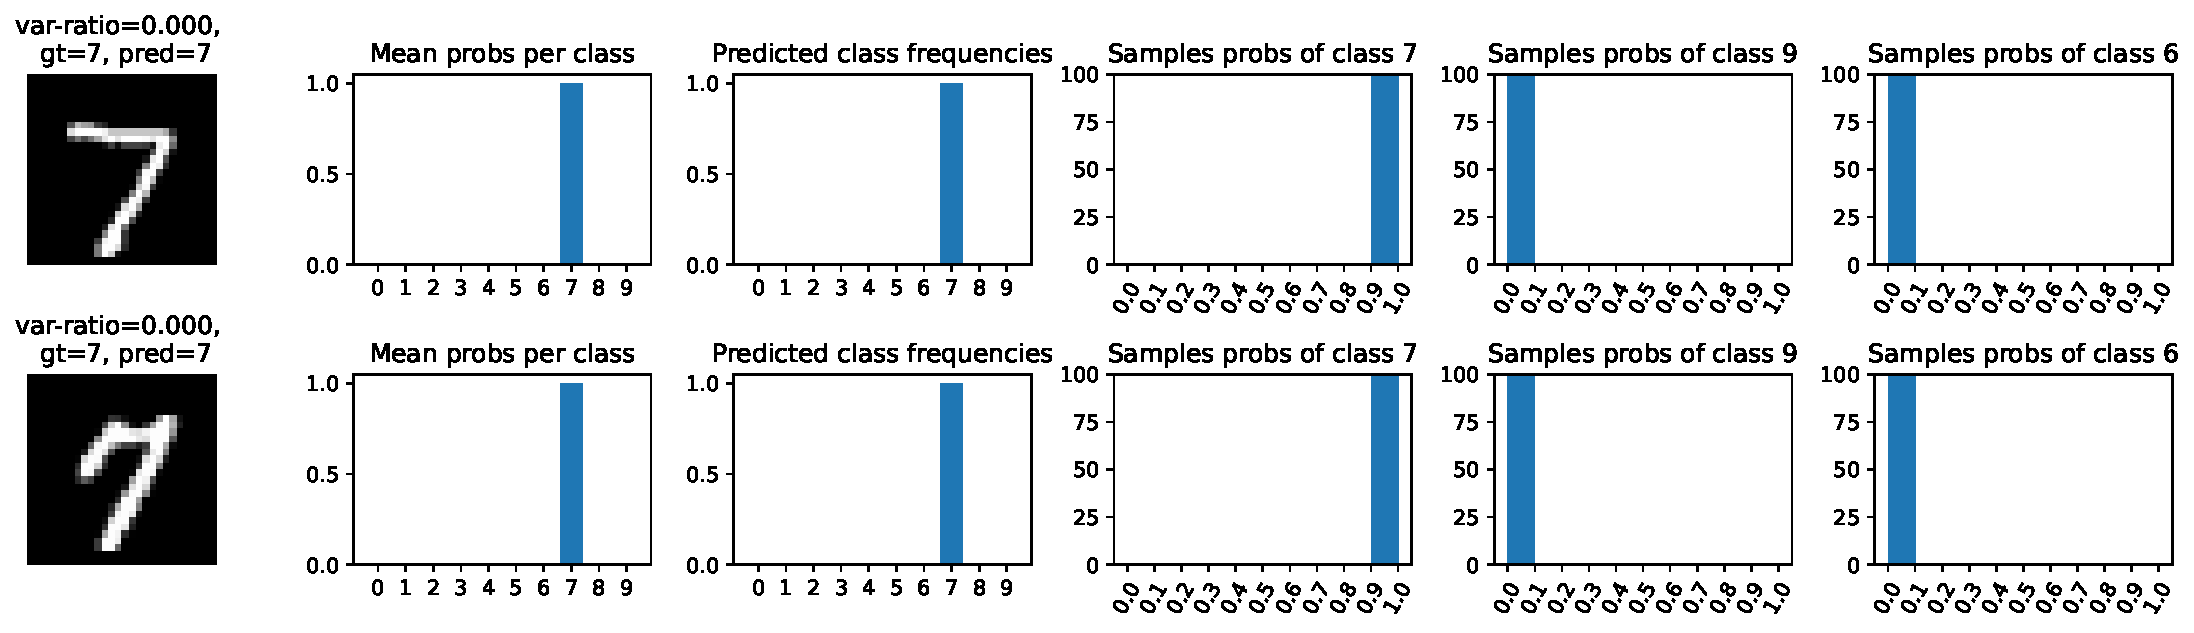
\includegraphics[width=0.95\textwidth]{var-ratio_certain_images.pdf}
    \caption{}
    \label{fig:varratio_certain}
\end{figure}
\begin{figure}[H]
    \centering
    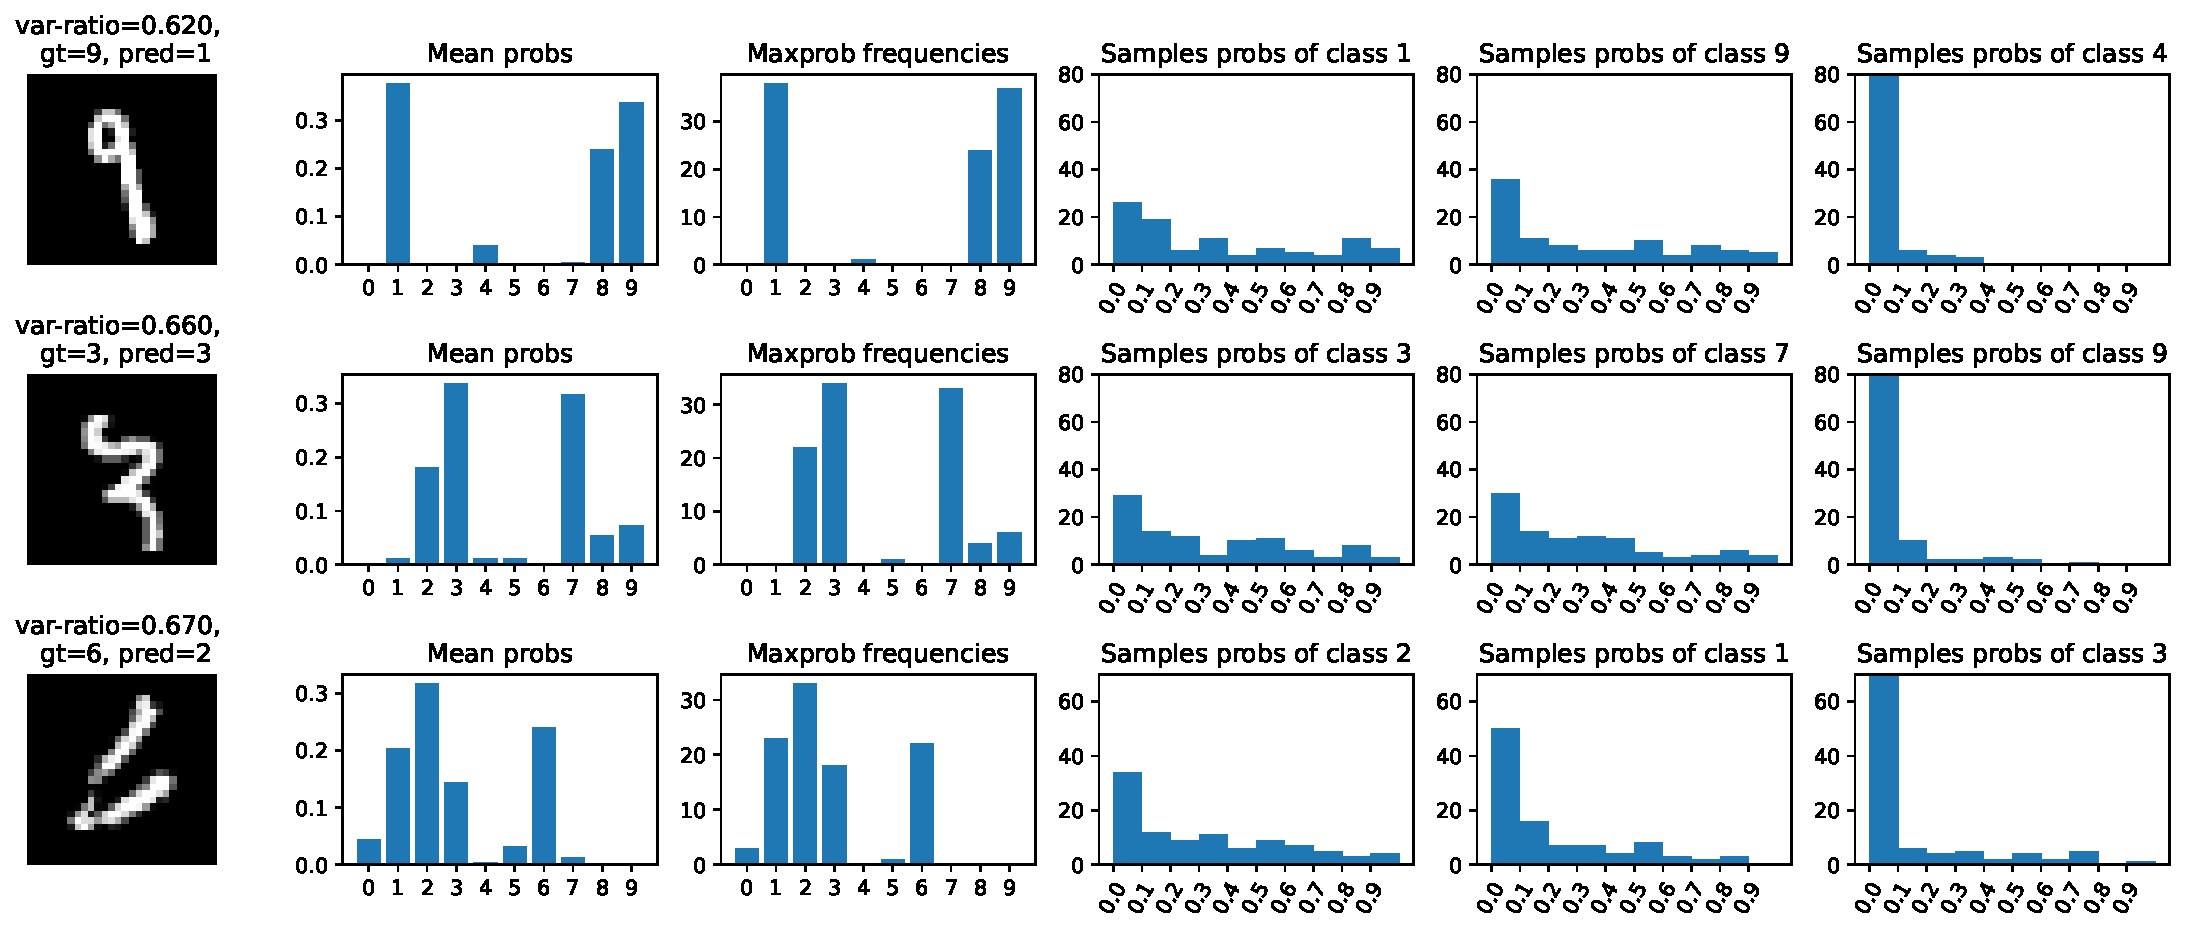
\includegraphics[width=0.95\textwidth]{var-ratio_uncertain_images.pdf}
    \caption{}
    \label{fig:varratio_uncertain}
\end{figure}

As we said when looking distribution of the mean of the probabilities of unconfident images, 

\section{Failure prediction}

\paragraph*{2.1. Compare the precision-recall curves of each method along with their AUPR values. Why did we use AUPR metric instead of standard AUROC?}

\begin{figure}[H]
    \centering
    \includegraphics[width=0.95\textwidth]{}
    \caption{}
    \label{fig:varratio_certain}
\end{figure}
\begin{figure}[H]
    \centering
    \includegraphics[width=0.95\textwidth]{}
    \caption{}
    \label{fig:varratio_uncertain}
\end{figure}


\section{Out-of-distribution detection}

\paragraph*{3.1. Compare the precision-recall curves of each OOD method along with their AUPR values. Which method perform best and why?}